\documentclass{article}
\usepackage[a4paper,
            top = 2in, 
            bottom = 1in, 
            left = 1in, 
            right=1in, 
            margin width = 1pt] {geometry}
\usepackage{amsfonts,amssymb,amsmath}
\usepackage{graphicx}
\usepackage{tikz}
\usepackage{subcaption}
\usepackage{array}
\usepackage{lipsum}
\usepackage{fancyhdr}
\usepackage{lmodern}
\usepackage{makecell} 
\usepackage{xcolor}
\usepackage{ragged2e}
\usepackage{enumitem}
\usepackage{newtxtext,newtxmath} 
\setlength{\parindent}{0pt}
\renewcommand{\baselinestretch}{1.35}
\usepackage{setspace}
\definecolor{ncertcyan}{HTML}{00B0F0}
\
\pagestyle{empty} % Start with empty page style
\thispagestyle{fancy} % Apply fancy style only to the first page
\renewcommand{\headrulewidth}{0pt} % Remove header rule
\fancyhead[L]{% Left header
        \includegraphics[width=8cm, height=1.7cm]{i.png} 
        }
\fancyhead[R]{% Right header
    Name: N.VaraLakshmi \\
    Batch: COMETFWC021 \\
    Date: 18 May 2025
}

\begin{document}
\begin{figure}[h]
    \centering
    \includegraphics[width=0.3\linewidth]{vennela.png}
\end{figure}
\begin{flushleft}
    \hspace{2em}
    {\color{ncertcyan}\fontsize{35pt}{30pt}\selectfont\textbf P\color{ncertcyan}\fontsize{22pt}{22pt}\selectfont\textbf {AIR OF}
    \color{ncertcyan}\fontsize{35pt}{30pt}\selectfont\textbf L\color{ncertcyan}\fontsize{22pt}{22pt}\selectfont\textbf {INEAR}
    \color{ncertcyan}\fontsize{35pt}{30pt}\selectfont\textbf E\color{ncertcyan}\fontsize{22pt}{22pt}\selectfont\textbf {QUATIONS}
    \vspace{0.5em}
    \\
    \hspace*{5.7em}
    \color{ncertcyan}\fontsize{22pt}{22pt}\selectfont\textbf {IN}
    \color{ncertcyan}\fontsize{35pt}{30pt}\selectfont\textbf T\color{ncertcyan}\fontsize{20pt}{20pt}\selectfont\textbf {WO}
    \color{ncertcyan}\fontsize{35pt}{30pt}\selectfont\textbf V\color{ncertcyan}\fontsize{22pt}{22pt}\selectfont\textbf {ARIABLES} }
    \end{flushleft}
\vspace{-2em}

\vspace{-6em}
\begin{flushright}
  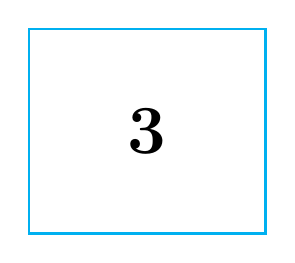
\begin{tikzpicture}
    \draw[ncertcyan, line width=1pt] (0,0) rectangle (3,2.6);
    \node at (1.5,1.3) {\color{black}\fontsize{68pt}{68pt}\selectfont\textbf{3}};
  \end{tikzpicture}
\end{flushright}


\vspace{-2em}
\noindent\textcolor{ncertcyan}{\rule{\linewidth}{5pt}}

\vspace{2em}
{ \noindent\color{ncertcyan}\fontsize{10pt}{10pt}\selectfont\textbf {3.1 Introduction}}
\vspace{0.5em}

{\fontsize{13}{16}\selectfont
\noindent
You must have come cross situations like the one given below.

\vspace{1em}
\hspace{1em}
Akhila went to a fair in her village. She wanted to enjoy rides on the Giant Wheel and play Hoopla (a game in which you throw a ring on the items kept in a stall, and if ring covers any object completely, you get it). The number of times she played Hoopla is half the number of rides she had on the Giant Wheel. If each ride costs  ₹3, and a game of Hoopla costs ₹4, how would you find out the number of rides she had and how many times she played Hoopla, provided she spent ₹20?
}

{\fontsize{13.75}{16}\selectfont
\vspace{1em}
\hspace{1em}
May be you will try it by considering different cases. If she has one ride, is it possible? Is it possible to have two rides? And so on. Or you may use the knowledge of Class IX to represent such situations as linear equations in two variables.
}
\vfill
\begin{center}
    2019--20
\end{center}
\newpage 
\pagestyle{fancy}
\fancyhf{} % Clear default headers/footers
\fancyhead[L]{\color{ncertcyan}{\large P\small AIR OF \large L\small INEAR \large E\small QUATIONS IN \large T\small WO \large V\small ARIABLES \large \hspace{18em}{39}}}
\fancyfoot[C]{\small 2019-20} % Centered footer
\renewcommand{\headrule}{\color{ncertcyan}\hrule height 3pt}

\setlength{\parindent}{1.5em}
\setlength{\parskip}{0pt}
\vspace{1em}
\begin{custom}
{\fontsize{12}{14.5}\selectfont

    \noindent Let us try this approach.
    
   \hspace{1.5em}
    Denote the number of rides that Akhila had by $x$, and the number of times she played Hoopla by $y$.Now the situation can be represented by two equations:
        \begin{align}
            y=\frac{1}{2}x\\
            3x+4y=20
            \end{align}
    
    \hspace{1.5em}    
    Can we find the solutions of this pair of equations? There are several ways of finding these,which will study in this chapter.

   
    \noindent \textbf{\textcolor{ncertcyan}{ \large P\large air OF \large L\large inear \large E\large quations in \large T\large wo \large V\large ariables}}

\justifying
\noindent
Recall, from Class IX, that the following are examples of linear equations in two variables:
\vspace{-1em}
\begin{align*}
    2x + 3y &= 5 \\
    x - 2y - 3 &= 0 \\
    \quad x - 0y &= 2, \text{ i.e., } x = 2
\end{align*}
\par
{You also know that an equation which can be put in the form $ax + by + c = 0$, where $a$, $b$ and $c$ are real numbers, and \textbf{a and b are not both zero}, is called a linear equation in two variables $x$ and $y$. (We often denote the condition $a$ and $b$ are not both zero by $a^2 + b^2 \neq 0$). You have also studied that a solution of such an equation is a pair of values, one for $x$ and the other for $y$, which makes the two sides of the equation equal.}

 For example, let us substitute $x = 1$ and $y = 1$ in the left hand side (LHS) of the equation $2x + 3y = 5$. Then
\vspace{-1em}
\[
\text{LHS} = 2(1) + 3(1) = 2 + 3 = 5,
\]

\hspace{6em}
which is equal to the right hand side (RHS) of the equation.

\hspace{6em}
Therefore, $x = 1$ and $y = 1$ is a solution of the equation $2x + 3y = 5$.

\hspace{6em}
Now let us substitute $x = 1$ and $y = 7$ in the equation $2x + 3y = 5$. Then,
\vspace{-2em}
\[
\text{LHS} = 2(1) + 3(7) = 2 + 21 = 23
\]
which is not equal to the RHS.

\noindent
Therefore, $x = 1$ and $y = 7$ is \textbf{not} a solution of the equation.

Geometrically, what does this mean? It means that the point $(1, 1)$ lies on the line representing the equation $2x + 3y = 5$, and the point $(1, 7)$ does not lie on it. So, \textbf{every solution of the equation is a point on the line representing it}.
}
\end{custom}
\newpage
\pagestyle{fancy}
\fancyhf{} % Clear default headers/footers
\fancyhead[L]{\color{ncertcyan}{\Large 40\hspace{25em}\Large M\small ATHEMATICS}}
\fancyfoot[C]{\small 2019-20} % Centered footer
\renewcommand{\headrule}{\color{ncertcyan}\hrule height 3pt}
\justifying
{\fontsize{12}{14.5}\selectfont 
\hspace{1.5em} In fact, this is true for any linear equation, that is, \textbf{each solution $(x, y)$ of a linear equation in two variables, $ax + by + c = 0$, corresponds to a point on the line representing the equation, and vice versa.}

\hspace{1.5em}Now, consider Equations (1) and (2) given above. These equations, \textbf{taken together}, represent the information we have about Akhila at the fair.

\hspace{1.5em} two linear equations are \textbf{in the same two variables $x$ and $y$}. Equations like these are called a \textbf{pair of linear equations in two variables}
\hspace{1.5em} Let us see what such pairs look like algebraically.

\hspace{1.5em} The general form for a pair of linear equations in two variables $x$ and $y$ is

\begin{center}
\begin{tabular}{ll}
    & $a_1x + b_1y + c_1 = 0$ \\
\text{and} & $a_2x + b_2y + c_2 = 0$,
\end{tabular}
\end{center}
\noindent
where $a_1, b_1, c_1, a_2, b_2, c_2$ are all real numbers and $a_1^2 + b_1^2 \ne 0, a_2^2 + b_2^2 \ne 0$.

\hspace{1.5em}Some examples of pair of linear equations in two variables are:

\begin{center}
$2x + 3y - 7 = 0$ & \text{and} $9x - 2y + 8 = 0$ \\
$5x = y$ & \text{and} $-7x + 2y + 3 = 0$ \\
$x + y = 7$ & \text{and} $17 = y$
\end{center}

\vspace{-1em}
\hspace{1.5em}Do you know, what do they look like geometrically?

\hspace{1.5em}Recall, that you have studied in Class IX that the geometrical (i.e., graphical) representation of a linear equation in two variables is a straight line. Can you now suggest what a pair of linear equations in two variables will look like, geometrically? There will be two straight lines, both to be considered together.

\hspace{1.5em}You have also studied in Class IX that given two lines in a plane, only one of the following three possibilities can happen:

\begin{enumerate}[label=(\roman*)]
    \item The two lines will intersect at one point.
    \item The two lines will not intersect, i.e., they are parallel.
    \item The two lines will be coincident.
\end{enumerate}
\noindent
We show all these possibilities in Fig. 3.1:

\begin{itemize}
    \item In Fig. 3.1 (a), they intersect.
    \item In Fig. 3.1 (b), they are parallel.
    \item In Fig. 3.1 (c), they are coincident.
\end{itemize}
}
\newpage
\begin{minipage}{0.3\textwidth}
    \includegraphics[width=\linewidth]{img11.jpg}
\end{minipage}
\hspace{0\textwidth}
\begin{minipage}{0.3\textwidth}
    \includegraphics[width=\linewidth]{img12.jpg} 
\end{minipage}
\begin{minipage}{0.3\textwidth}
    \includegraphics[width=\linewidth]{img13.jpg}
\end{minipage}

{\fontsize{13}{16}\selectfont
Both ways of representing a pair oflinear equations go hand-in-hand-the algebrabic and the geometric ways.Let us consider some examples.
\vspace{1em}

\noindent
\textcolor{ncertcyan}{Example 1:}Let us take the example given in section 3.1.Akhila goes to a fair with 20 and want to have rides on the Giant Wheel and play Hoopla.Represent this situation algebraically and graphically(geometrically).\\
\textcolor{ncertcyan}{solution:}The pair of equations formed is:}
  \begin{equation*}
y=\frac{1}{2}x
  \end{equation*}
i.e,,
   \begin{align}
x-2y=0 \\
3x+4y=20
   \end{align}

\vspace{-1em}
{\fontsize{13}{16}\selectfont Let us represnt these equations graphically,For this,we need at least two solutions for \\
each equation.We give these solutions in Table3.1.}

\center \textcolor{ncertcyan}{\large Table 3.1}

\begin{minipage}{0.3\textwidth}
    \includegraphics[width=\linewidth]{img15.jpg}
\end{minipage}
\hspace{0.05\textwidth}
\begin{minipage}{0.5\textwidth}
    \includegraphics[width=\linewidth]{img14.jpg} 
\end{minipage}

\justify
{\fontsize{13}{16}\selectfont 
\hspace{1em}Recall from class IX that there are infinitely many solutions of each linear equation.so each of you can choose any 
two values,which may not be the ones we have chosen.Can tou guess why we have chosen x=0 in the first equation and in the second equation?when one of the variable is zero,the equation reduces to a linear.}
\end{document}
